\documentclass[aspectratio=169,12pt,t]{beamer}

% --- Theme: Metropolis (modern, clean) ---
\usetheme[progressbar=frametitle,numbering=fraction,block=fill]{metropolis}

% --- Fira Sans font (install texlive-fonts-extra if missing) ---
\IfFileExists{FiraSans.sty}{\usepackage[sfdefault]{FiraSans}}{}

% --- Light background with warm accent ---
\definecolor{mDarkTeal}{RGB}{35,55,59}
\definecolor{mLightBrown}{RGB}{235,228,216}
\definecolor{mAccent}{RGB}{140,70,20}

\setbeamercolor{normal text}{fg=mDarkTeal,bg=white}
\setbeamercolor{alerted text}{fg=mAccent}
\setbeamercolor{frametitle}{bg=mDarkTeal,fg=white}
\setbeamercolor{progress bar}{fg=mAccent,bg=mLightBrown}
\setbeamercolor{title separator}{fg=mAccent}
\setbeamercolor{progress bar in head/foot}{fg=mAccent,bg=mLightBrown}
\setbeamercolor{progress bar in section page}{fg=mAccent,bg=mLightBrown}

% --- Packages ---
\usepackage[utf8]{inputenc}
\usepackage{amsmath,amssymb,amsthm}
\usepackage{mathrsfs}
\usepackage{tikz}
\usetikzlibrary{arrows.meta,positioning,calc,decorations.pathreplacing,shapes,patterns,shadows}
\usepackage{pgfplots}
\pgfplotsset{compat=1.18}

% --- Semi-transparent white highlight for text on top of background images ---
\usepackage[most]{tcolorbox}

% Inline highlight: \hl{short text}
\newtcbox{\hl}{%
  nobeforeafter, tcbox raise base,
  colback=white, opacityback=0.6,
  colframe=white, opacityframe=0,
  sharp corners, boxsep=2pt, left=3pt, right=3pt, top=2pt, bottom=2pt%
}

% Block highlight: \begin{hlbox} ... \end{hlbox}  (multi-line, paragraphs, itemize)
\newtcolorbox{hlbox}[1][]{%
  enhanced, breakable,
  colback=white, opacityback=0.6,
  colframe=white, opacityframe=0,
  boxsep=3pt, left=6pt, right=6pt, top=4pt, bottom=4pt,
  sharp corners,
  {#1}%
}

% --- Custom colors for content types ---
\definecolor{defcolor}{RGB}{25,85,120}
\definecolor{thmcolor}{RGB}{140,35,35}
\definecolor{proofcolor}{RGB}{35,100,50}
\definecolor{excolor}{RGB}{140,75,10}
\definecolor{remcolor}{RGB}{90,90,90}

% --- Beamer blocks for mathematical content types (semi-transparent) ---
\tcbset{hlblockbase/.style={
  enhanced, breakable,
  coltitle=white, fonttitle=\bfseries,
  opacitybacktitle=0.8, opacityback=0.6,
  opacityframe=0,
  sharp corners,
  boxsep=1pt, left=5pt, right=5pt, top=2pt, bottom=2pt,
  toptitle=1pt, bottomtitle=1pt
}}

\newtcolorbox{defblock}[1]{hlblockbase, title={#1},
  colbacktitle=defcolor, colback=defcolor!15, colframe=defcolor}
\newtcolorbox{thmblock}[1]{hlblockbase, title={#1},
  colbacktitle=thmcolor, colback=thmcolor!15, colframe=thmcolor}
\newtcolorbox{proofblock}[1]{hlblockbase, title={#1},
  colbacktitle=proofcolor, colback=proofcolor!15, colframe=proofcolor}
\newtcolorbox{exblock}[1]{hlblockbase, title={#1},
  colbacktitle=excolor, colback=excolor!15, colframe=excolor}
\newtcolorbox{remblock}[1]{hlblockbase, title={#1},
  colbacktitle=remcolor, colback=remcolor!15, colframe=remcolor}

% --- Metadata ---
\title{Chapter 3: Numerical Sequences and Series}
\subtitle{Section: Rearrangements}
\author{Based on Walter Rudin's \emph{Principles of Mathematical Analysis}}
\date{}

\begin{document}

% =============================================================================
% TITLE AND OUTLINE
% =============================================================================
{
\usebackgroundtemplate{%
  
\includegraphics[width=\paperwidth,height=\paperheight,keepaspectratio=false]{chapter_03_bg_00.png}%
}
\begin{frame}[plain]
  \titlepage
  \note{
    Welcome to the final section of Chapter 3 of Principles of Mathematical
    Analysis. We close our study of series with a question that sounds
    almost silly: if we add up the same numbers in a different order, can
    the answer change? For finite sums the answer is obviously no. For
    infinite series the answer is one of the most surprising facts in all
    of analysis. We will see a concrete example where reordering changes
    the sum, then prove Riemann's rearrangement theorem, which says that a
    conditionally convergent series can be rearranged to do essentially
    anything we want. Finally we will prove that absolutely convergent
    series are completely immune to reordering. Let's dive in.
  }
\end{frame}
}

{
\usebackgroundtemplate{%
  
\includegraphics[width=\paperwidth,height=\paperheight,keepaspectratio=false]{chapter_03_bg_01.png}%
}
\begin{frame}[c]{Outline}
  \begin{center}
    \tableofcontents
  \end{center}
  \note{
    Here is the plan. We start with some motivation, contrasting finite
    sums, where order never matters, with infinite series, where the order
    of the terms is built into the very definition of the sum. Then
    Definition 3.52 makes the notion of a rearrangement precise. Example
    3.53 gives a concrete rearrangement of the alternating harmonic series
    that converges to a different value. The centerpiece is Riemann's
    rearrangement theorem, Theorem 3.54: a conditionally convergent real
    series can be rearranged so that its partial sums have any prescribed
    upper and lower limits. We then prove Theorem 3.55, which says
    absolutely convergent series can be reordered freely, and we finish
    with a summary of the section and of the whole chapter.
  }
\end{frame}

% =============================================================================
\section{Motivation}
% =============================================================================

% --- Build 1/3 ---
\begin{frame}{Does the Order of Summation Matter?}
  \begin{hlbox}
  \begin{itemize}
    \item For \alert{finite} sums, order never matters:
      $a + b + c = c + a + b$ \quad (commutativity + associativity)
  \end{itemize}
  \end{hlbox}

  \note{
    Let us begin with the basic question of this section: does the order in
    which we add numbers matter? For finite sums, certainly not. Addition
    is commutative and associative, so any reordering of finitely many
    terms produces exactly the same total. This is so familiar that we
    never think about it. The surprise is what happens when we pass from
    finitely many terms to infinitely many.
  }
\end{frame}

% --- Build 2/3 ---
\begin{frame}{Does the Order of Summation Matter?}
  \begin{hlbox}
  \begin{itemize}
    \item For \alert{finite} sums, order never matters:
      $a + b + c = c + a + b$ \quad (commutativity + associativity)
    \item An infinite series is \emph{not} just a set of numbers:
      \[
        \sum a_n = \lim_{N \to \infty} s_N, \qquad s_N = a_1 + a_2 + \cdots + a_N
      \]
      The \alert{order of the terms} determines the partial sums!
  \end{itemize}
  \end{hlbox}

  \note{
    But an infinite series is not just a bag of numbers. By definition, its
    sum is the limit of the partial sums, and the partial sums are formed
    by adding the terms in a specific order: first "a" sub 1, then "a" sub
    2, and so on. Change the order of the terms and you change every
    partial sum, hence you change the sequence whose limit defines the sum.
    There is no obvious reason the new limit should equal the old one, or
    even exist.
  }
\end{frame}

% --- Build 3/3 ---
\begin{frame}{Does the Order of Summation Matter?}
  \begin{hlbox}
  \begin{itemize}
    \item For \alert{finite} sums, order never matters:
      $a + b + c = c + a + b$ \quad (commutativity + associativity)
    \item An infinite series is \emph{not} just a set of numbers:
      \[
        \sum a_n = \lim_{N \to \infty} s_N, \qquad s_N = a_1 + a_2 + \cdots + a_N
      \]
      The \alert{order of the terms} determines the partial sums!
    \item Do reordered series still \alert{converge}?
      If so, to the \alert{same sum}?
  \end{itemize}
  \end{hlbox}

  \note{
    So we face two natural questions. First, if a series converges, does
    every reordering of it still converge? Second, if a reordering does
    converge, must it converge to the same sum? The answers form a
    beautiful dichotomy. For series that converge absolutely, reordering
    changes nothing. For series that converge only conditionally,
    reordering can change everything, and Riemann's theorem will tell us
    exactly how badly. First, let us make the idea of reordering precise.
  }
\end{frame}
}

{
\usebackgroundtemplate{%
  
\includegraphics[width=\paperwidth,height=\paperheight,keepaspectratio=false]{chapter_03_bg_02.png}%
}
% =============================================================================
\section{What Is a Rearrangement?}
% =============================================================================

% --- Build 1/2 ---
\begin{frame}{Definition 3.52: Rearrangement}
  \begin{defblock}{Definition 3.52}
    Let $\{k_n\}$, $n = 1, 2, 3, \dots$, be a sequence in which every
    positive integer appears \alert{once and only once}
    ($\{k_n\}$ is a 1--1 function from $J$ onto $J$; see Definition 2.2).
    Putting
    \[
      a'_n = a_{k_n} \qquad (n = 1, 2, 3, \dots),
    \]
    we say that $\Sigma a'_n$ is a \alert{rearrangement} of $\Sigma a_n$.
  \end{defblock}

  \note{
    Here is the precise definition. A rearrangement is described by a
    sequence "k" sub "n" in which every positive integer appears exactly
    once; in other words, a one to one function from the positive integers
    onto the positive integers, a permutation. The new series has term
    number "n" equal to "a" sub "k" sub "n". The phrase once and only once
    is the heart of the matter: it guarantees that no term is dropped and
    none is repeated, so the rearranged series really is built from the
    same ingredients, just served in a different order. That is exactly
    what makes our question a fair one. Let us draw a picture of this.
  }
\end{frame}

% --- Build 2/2 ---
\begin{frame}{Definition 3.52: Rearrangement}
  \vspace{0.4em}
  \begin{center}
  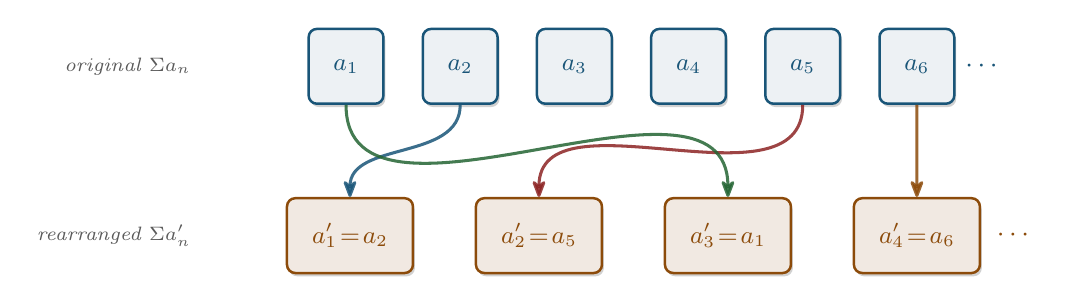
\begin{tikzpicture}[
    >={Stealth[round]},
    softshadow/.style={drop shadow={opacity=0.18, shadow xshift=0.7pt,
       shadow yshift=-1.2pt, fill=black}},
    orig/.style={draw=defcolor, line width=0.9pt, rounded corners=3pt,
       fill=defcolor!8, text=defcolor, minimum size=9.5mm, font=\small, softshadow},
    rear/.style={draw=excolor, line width=0.9pt, rounded corners=3pt,
       fill=excolor!12, text=excolor, minimum width=16mm, minimum height=9.5mm,
       font=\small, softshadow},
    rowlbl/.style={font=\scriptsize\itshape, text=remcolor, anchor=east},
    link/.style={line width=1.1pt, -{Stealth[round]}, opacity=0.85}
  ]
    % Row labels
    \node[rowlbl] at (1.05, 2.15) {original $\Sigma a_n$};
    \node[rowlbl] at (1.05, 0)    {rearranged $\Sigma a'_n$};

    % Original terms
    \foreach \i in {1,...,6} {
      \node[orig] (a\i) at (1.45 + 1.45*\i, 2.15) {$a_{\i}$};
    }
    \node[defcolor] at (11.0, 2.15) {$\cdots$};

    % Rearranged terms (a permutation of the same boxes)
    \node[rear] (b1) at (2.95, 0)  {$a'_1\!=\!a_2$};
    \node[rear] (b2) at (5.35, 0)  {$a'_2\!=\!a_5$};
    \node[rear] (b3) at (7.75, 0)  {$a'_3\!=\!a_1$};
    \node[rear] (b4) at (10.15, 0) {$a'_4\!=\!a_6$};
    \node[excolor] at (11.4, 0) {$\cdots$};

    % Colour-coded curved links showing where each term goes
    \draw[link, defcolor]  (a2.south) to[out=-90,in=90] (b1.north);
    \draw[link, thmcolor]  (a5.south) to[out=-90,in=90] (b2.north);
    \draw[link, proofcolor](a1.south) to[out=-90,in=90] (b3.north);
    \draw[link, excolor]   (a6.south) to[out=-90,in=90] (b4.north);
  \end{tikzpicture}
  \end{center}

  \begin{center}
    \begin{hlbox}
    \footnotesize\itshape
    $\{k_n\}=(2,5,1,6,\dots)$ is a bijection of $J$ onto itself --- a
    \textbf{permutation} of the same terms.
    \end{hlbox}
  \end{center}

  \begin{hlbox}
  \textbf{Same terms, new order} $\Rightarrow$ partial sums $\{s_n\}$ and
  $\{s'_n\}$ consist of \alert{entirely different numbers} in general.
  \end{hlbox}

  \note{
    The picture shows what a rearrangement does. The blue boxes on the top
    row are the original terms in their original order. The amber boxes on
    the bottom row are the rearranged terms: here "a" prime sub 1 is "a"
    sub 2, "a" prime sub 2 is "a" sub 5, and so on. Each colored arrow
    traces a single term down to its new position, and the crossing of the
    arrows is exactly the shuffling. The caption records that the index
    sequence "k" sub "n" is a bijection, a permutation, so every box is
    used once and only once. The line at the bottom records the key
    consequence: the partial sums of the two series consist, in general,
    of entirely different numbers. A concrete example will show that
    things really can go wrong.
  }
\end{frame}
}

{
\usebackgroundtemplate{%
  
\includegraphics[width=\paperwidth,height=\paperheight,keepaspectratio=false]{chapter_03_bg_03.png}%
}
% =============================================================================
\section{A Cautionary Example}
% =============================================================================

% --- Build 1/4 ---
\begin{frame}{Example 3.53: Reordering the Alternating Harmonic Series}
  \begin{exblock}{Example 3.53}
    The alternating harmonic series converges (Theorem 3.43):
    \begin{equation}
      1 - \tfrac{1}{2} + \tfrac{1}{3} - \tfrac{1}{4} + \tfrac{1}{5} - \tfrac{1}{6} + \cdots \tag{22}
    \end{equation}
    Consider the rearrangement
    \emph{(two positive terms, then one negative)}:
    \begin{equation}
      1 + \tfrac{1}{3} - \tfrac{1}{2} + \tfrac{1}{5} + \tfrac{1}{7} - \tfrac{1}{4}
        + \tfrac{1}{9} + \tfrac{1}{11} - \tfrac{1}{6} + \cdots \tag{23}
    \end{equation}
  \end{exblock}

  \note{
    Here is the classic example. Equation 22 is the alternating harmonic
    series: one, minus one half, plus one third, minus one fourth, and so
    on. It converges by the alternating series test, Theorem 3.43, but it
    does not converge absolutely, since the harmonic series diverges.
    Equation 23 is a rearrangement of it: we take two positive terms, then
    one negative term, and repeat. So it starts one, plus one third, minus
    one half, then one fifth, plus one seventh, minus one fourth, and so
    on. Every term of the original series appears exactly once. We will
    now show that this innocent looking reshuffle changes the sum.
  }
\end{frame}

% --- Build 2/4 ---
\begin{frame}{Example 3.53: Reordering the Alternating Harmonic Series}
  \begin{hlbox}
  \textbf{Step 1: The original sum $s$ satisfies $s < \frac{5}{6}$.}
  \[
    s = \underbrace{1 - \tfrac{1}{2} + \tfrac{1}{3}}_{= 5/6}
      \underbrace{- \tfrac{1}{4} + \tfrac{1}{5}}_{< 0}
      \underbrace{- \tfrac{1}{6} + \tfrac{1}{7}}_{< 0} - \cdots
    \;\Longrightarrow\; \boxed{s < 1 - \tfrac{1}{2} + \tfrac{1}{3} = \tfrac{5}{6}}
  \]
  \end{hlbox}

  \note{
    First we pin down the true sum of the original series, called "s"; we
    will need it as a benchmark to compare the rearrangement against. Group
    the series the way the slide does. The first three terms add up to
    exactly five sixths. Everything after that falls into pairs: minus one
    fourth plus one fifth, then minus one sixth plus one seventh, and so
    on, and each pair is negative because its negative term has the larger
    absolute value. So "s" is five sixths plus a whole string of negative
    corrections, which forces the boxed conclusion: "s" is strictly less
    than five sixths. Hold on to that number, and let us turn to the
    rearrangement.
  }
\end{frame}

% --- Build 3/4 ---
\begin{frame}{Example 3.53: Reordering the Alternating Harmonic Series}
  \begin{hlbox}
  \textbf{Step 2: The rearranged partial sums $s'_{3k}$ increase.}

  Group (23) into triples; the $k$th triple is
  \[
    \frac{1}{4k-3} + \frac{1}{4k-1} - \frac{1}{2k} > 0 \qquad (k \geq 1),
  \]
  so
  \[
    s'_3 < s'_6 < s'_9 < \cdots, \qquad s'_3 = 1 + \tfrac{1}{3} - \tfrac{1}{2} = \tfrac{5}{6}.
  \]
  \end{hlbox}

  \note{
    Now look at the rearranged series in blocks of three: two positive
    terms, then one negative. The slide shows that every such block, the
    "k"-th one, is positive. Here is why: both positive fractions in the
    block are larger than one over four "k", so the two of them together
    exceed one over two "k", which is exactly the negative term being
    subtracted. The positives win, and each block contributes a net
    positive amount. So the running total taken right after each complete
    block keeps climbing, forming a strictly increasing sequence, and the
    very first of these totals already equals five sixths. Intuitively,
    serving two positive terms for every negative one front-loads the
    positive mass and props the sum up.
  }
\end{frame}

% --- Build 4/4 ---
\begin{frame}{Example 3.53: Reordering the Alternating Harmonic Series}
  \begin{hlbox}
  \textbf{Step 3: Conclusion.}
  \[
    \limsup_{n \to \infty} s'_n > s'_3 = \tfrac{5}{6} > s
  \]
  \end{hlbox}

  \begin{remblock}{The rearrangement changes the sum}
    Series (23) does \alert{not} converge to $s$.\\
    (It does converge --- in fact to $\tfrac{3}{2}\ln 2$, while $s = \ln 2$.)
  \end{remblock}

  \note{
    Putting the two steps together: the upper limit of the rearranged
    partial sums is greater than "s" prime sub 3, which equals five
    sixths, while the original sum "s" is strictly less than five sixths.
    So the rearranged series certainly does not converge to "s". As the
    remark notes, the rearrangement does still converge; Rudin leaves the
    verification to the reader. As a piece of extra insight beyond the
    book: the original sum is the natural logarithm of 2, about 0.69, and
    the rearranged sum is three halves times the natural logarithm of 2,
    about 1.04. Reordering inflated the sum by exactly fifty percent! A
    picture makes this vivid.
  }
\end{frame}

\begin{frame}{The Two Series, Side by Side}
  \begin{center}
  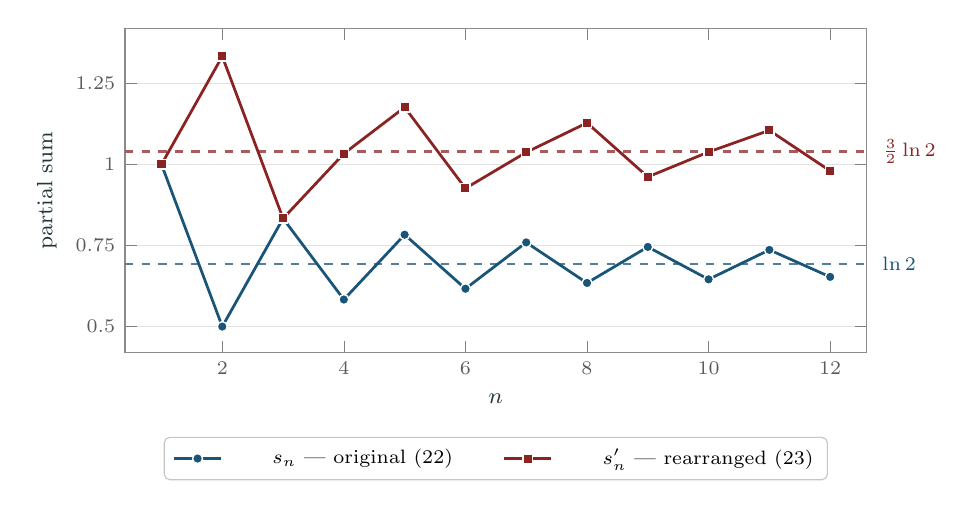
\begin{tikzpicture}
    \begin{axis}[
      width=11cm, height=5.7cm,
      xlabel={$n$}, ylabel={partial sum},
      xmin=0.4, xmax=12.6, ymin=0.42, ymax=1.42,
      axis line style={remcolor!70},
      x axis line style={-{Stealth[round]}},
      y axis line style={-{Stealth[round]}},
      label style={font=\footnotesize, text=mDarkTeal},
      tick label style={font=\scriptsize, text=remcolor},
      xtick={2,4,6,8,10,12},
      ytick={0.5,0.75,1.0,1.25},
      ymajorgrids=true, grid style={remcolor!18, line width=0.4pt},
      legend style={font=\scriptsize, draw=remcolor!35, fill=white,
        rounded corners=2pt, at={(0.5,-0.26)}, anchor=north,
        legend columns=2, column sep=1.6em},
      clip=false,
    ]
      % Asymptotic limits (drawn first, behind the data)
      \addplot[defcolor!75, dashed, line width=0.8pt, forget plot, domain=0.4:12.6] {0.6931};
      \addplot[thmcolor!75, dashed, line width=0.8pt, forget plot, domain=0.4:12.6] {1.0397};
      % Original alternating harmonic partial sums
      \addplot[defcolor, line width=1pt, mark=*, mark size=1.8pt,
        mark options={fill=defcolor, draw=white, line width=0.5pt}] coordinates {
        (1,1.0000) (2,0.5000) (3,0.8333) (4,0.5833) (5,0.7833) (6,0.6167)
        (7,0.7595) (8,0.6345) (9,0.7456) (10,0.6456) (11,0.7365) (12,0.6532)
      };
      \addlegendentry{$s_n$ --- original (22)}
      % Rearranged partial sums
      \addplot[thmcolor, line width=1pt, mark=square*, mark size=1.7pt,
        mark options={fill=thmcolor, draw=white, line width=0.5pt}] coordinates {
        (1,1.0000) (2,1.3333) (3,0.8333) (4,1.0333) (5,1.1762) (6,0.9262)
        (7,1.0373) (8,1.1282) (9,0.9615) (10,1.0384) (11,1.1051) (12,0.9801)
      };
      \addlegendentry{$s'_n$ --- rearranged (23)}
      % Limit labels in the right margin (clip=false keeps them clear of data)
      \node[thmcolor, font=\scriptsize, anchor=west] at (axis cs:12.7,1.0397)
        {$\tfrac{3}{2}\ln 2$};
      \node[defcolor, font=\scriptsize, anchor=west] at (axis cs:12.7,0.6931)
        {$\ln 2$};
    \end{axis}
  \end{tikzpicture}
  \end{center}

  \note{
    This plot shows the first twelve partial sums of both series. The blue
    dots are the partial sums of the original alternating harmonic series,
    equation 22; they oscillate and squeeze down toward the blue dashed
    line at the natural logarithm of 2, roughly 0.69. The red squares are
    the partial sums of the rearrangement, equation 23. Same terms, but
    because two positive terms arrive for every negative one, the red
    sequence settles around the higher red dashed line, at three halves
    times the natural logarithm of 2, roughly 1.04. The two series use
    identical ingredients and converge to different sums. Riemann turned
    this observation into a spectacular general theorem.
  }
\end{frame}
}

{
\usebackgroundtemplate{%
  
\includegraphics[width=\paperwidth,height=\paperheight,keepaspectratio=false]{chapter_03_bg_04.png}%
}
% =============================================================================
\section{Riemann's Rearrangement Theorem}
% =============================================================================

\begin{frame}{Theorem 3.54: Riemann's Rearrangement Theorem}
  \begin{thmblock}{Theorem 3.54 (Riemann)}
    Let $\Sigma a_n$ be a series of \emph{real} numbers which converges,
    but \alert{not absolutely}. Suppose
    \[
      -\infty \leq \alpha \leq \beta \leq \infty.
    \]
    Then there exists a rearrangement $\Sigma a'_n$ with partial sums
    $s'_n$ such that
    \begin{equation}
      \liminf_{n \to \infty} s'_n = \alpha, \qquad
      \limsup_{n \to \infty} s'_n = \beta. \tag{24}
    \end{equation}
  \end{thmblock}

  \note{
    Here is the remarkable theorem, due to Riemann. Take any series of
    real numbers that converges, but not absolutely; we call such series
    conditionally convergent. Pick any two extended real numbers alpha and
    beta with alpha less than or equal to beta; they are even allowed to
    be plus or minus infinity. Then there is a rearrangement of the series
    whose partial sums have lower limit exactly alpha and upper limit
    exactly beta. In other words, by merely reordering the terms, we have
    total control over the limiting behavior of the partial sums. The
    hidden reason this works, which the proof will make precise, is that a
    conditionally convergent series secretly carries an infinite amount of
    positive material and an infinite amount of negative material; we
    simply dole them out in whatever proportion steers the sum where we
    please. Let us spell out what this freedom buys us.
  }
\end{frame}

% --- Build 1/3 ---
\begin{frame}{What the Theorem Gives Us}
  \begin{remblock}{Conditional convergence: anything goes}
    For a conditionally convergent real series, rearrangements exist that:
    \begin{itemize}
      \item converge to \alert{any prescribed sum} $\;$
        (take $\alpha = \beta = $ your number)
    \end{itemize}
  \end{remblock}

  \note{
    Let us unpack the statement, one choice of alpha and beta at a time.
    If we choose alpha equal to beta equal to some number, the rearranged
    partial sums have the same lower and upper limit, so the rearrangement
    converges, and it converges exactly to that number. In other words,
    by reordering alone we can make a conditionally convergent series add
    up to any target we like. And that is only the first option.
  }
\end{frame}

% --- Build 2/3 ---
\begin{frame}{What the Theorem Gives Us}
  \begin{remblock}{Conditional convergence: anything goes}
    For a conditionally convergent real series, rearrangements exist that:
    \begin{itemize}
      \item converge to \alert{any prescribed sum} $\;$
        (take $\alpha = \beta = $ your number)
      \item diverge to $+\infty$ or to $-\infty$ $\;$
        (take $\alpha = \beta = \pm\infty$)
    \end{itemize}
  \end{remblock}

  \note{
    Second, the targets are allowed to be infinite. Choosing alpha and
    beta both equal to plus infinity forces the partial sums to march off
    to plus infinity, so the rearranged series diverges; choosing both
    equal to minus infinity sends it to minus infinity instead. A
    convergent series has been reordered into a divergent one. There is
    one more behavior on the menu.
  }
\end{frame}

% --- Build 3/3 ---
\begin{frame}{What the Theorem Gives Us}
  \begin{remblock}{Conditional convergence: anything goes}
    For a conditionally convergent real series, rearrangements exist that:
    \begin{itemize}
      \item converge to \alert{any prescribed sum} $\;$
        (take $\alpha = \beta = $ your number)
      \item diverge to $+\infty$ or to $-\infty$ $\;$
        (take $\alpha = \beta = \pm\infty$)
      \item \alert{oscillate} between any two prescribed bounds
        (take $\alpha < \beta$)
    \end{itemize}
  \end{remblock}

  \note{
    Finally, if alpha is strictly less than beta, the partial sums settle
    into permanent oscillation, dipping arbitrarily close to alpha and
    climbing arbitrarily close to beta, forever. So conditional
    convergence is extremely fragile: the sum of such a series is an
    artifact of the order of its terms. Now let us see how the proof
    achieves all this.
  }
\end{frame}

\begin{frame}{Proof Strategy: Theorem 3.54}
  \begin{hlbox}
  \textbf{Goal:} Rearrange $\Sigma a_n$ so that
  $\liminf s'_n = \alpha$ and $\limsup s'_n = \beta$.

  \vspace{0.6em}
  \textbf{Approach:}
  \begin{enumerate}
    \item Split the series into its positive part and negative part;
      show \alert{both diverge}.
    \item Choose target sequences $\alpha_n \to \alpha$, $\beta_n \to \beta$.
    \item \alert{Greedy construction:} add positive terms until the sum
      exceeds $\beta_1$; add negative terms until it drops below $\alpha_1$;
      repeat with $\beta_2$, $\alpha_2$, \dots
    \item Overshoots are bounded by single terms, and the terms tend to $0$
      --- so the turning points converge to $\beta$ and $\alpha$.
  \end{enumerate}
  \end{hlbox}

  \note{
    Before the formal proof, here is the high level plan. Step 1 is the
    key structural fact: in a conditionally convergent series, the
    positive terms alone form a divergent series, and so do the negative
    terms. This gives us two infinite reservoirs: one that can push the
    partial sums up as far as we like, and one that can pull them down as
    far as we like. Step 2 picks finite targets, alpha sub "n" and beta
    sub "n", marching toward alpha and beta. Step 3 is a greedy
    construction: we alternate between the reservoirs, each time taking
    just enough terms to cross the current target. Step 4 explains why
    this works: each overshoot is at most the size of the last term used,
    and the terms of a convergent series tend to zero, so the overshoots
    vanish. Let us carry this out.
  }
\end{frame}

% --- Build 1/2 ---
\begin{frame}{Proof of Theorem 3.54 --- Step 1: Positive and Negative Parts}
  \begin{proofblock}{Step 1: Split $a_n$ into positive and negative parts}
    For $n = 1, 2, 3, \dots$ put
    \[
      p_n = \frac{|a_n| + a_n}{2}, \qquad q_n = \frac{|a_n| - a_n}{2}.
    \]
    Then
    \[
      p_n - q_n = a_n, \qquad p_n + q_n = |a_n|, \qquad p_n \geq 0, \qquad q_n \geq 0.
    \]
  \end{proofblock}

  \note{
    We start by splitting each term into a positive part and a negative
    part. The quantity "p" sub "n" is the positive part: it equals "a" sub
    "n" when that term is positive, and zero when the term is negative. The
    quantity "q" sub "n" is the size of the negative part: zero when "a"
    sub "n" is positive, and the absolute value of "a" sub "n" when it is
    negative. The two formulas on the slide, written with absolute values,
    are just a compact way to say exactly that. From them we read off the
    identities: the difference of the parts recovers "a" sub "n", their sum
    recovers the absolute value, and neither part is ever negative. Next we
    show that both of these series diverge.
  }
\end{frame}

% --- Build 2/2 ---
\begin{frame}{Proof of Theorem 3.54 --- Step 1: Positive and Negative Parts}
  \begin{proofblock}{Step 1 (continued): $\Sigma p_n$ and $\Sigma q_n$ both diverge}
    \begin{itemize}
      \item If \emph{both} converged: $\Sigma (p_n + q_n) = \Sigma |a_n|$
        would converge --- but $\Sigma a_n$ is \alert{not} absolutely convergent.
      \item If \emph{exactly one} converged: from
        $\sum_{n=1}^{N} a_n = \sum_{n=1}^{N} p_n - \sum_{n=1}^{N} q_n$,
        $\Sigma a_n$ would diverge --- but $\Sigma a_n$ \alert{converges}.
    \end{itemize}
  \end{proofblock}

  \begin{hlbox}
  \textbf{Technique:} proof by contradiction, twice --- using \emph{both}
  hypotheses.
  \end{hlbox}

  \note{
    Now the crucial claim: the series of "p" sub "n" and the series of
    "q" sub "n" must both diverge, and each hypothesis rules out one
    failure mode. If both converged, their sum, the series of absolute
    values, would converge, contradicting that our series is not
    absolutely convergent. If exactly one converged, look at the identity
    on the slide: the partial sum of "a" sub "n" is the partial sum of
    the "p" terms minus that of the "q" terms, so the series of "a" sub
    "n" would diverge, contradicting convergence. Conditional convergence
    is exactly the sweet spot where both reservoirs are infinite.
  }
\end{frame}

\begin{frame}{Proof of Theorem 3.54 --- Step 2: The Two Reservoirs}
  \begin{proofblock}{Step 2: Collect the terms by sign}
    \begin{itemize}
      \item $P_1, P_2, P_3, \dots$ = the \alert{nonnegative} terms of
        $\Sigma a_n$, in their original order
      \item $Q_1, Q_2, Q_3, \dots$ = the \alert{absolute values of the
        negative} terms, in their original order
    \end{itemize}
    $\Sigma P_n$, $\Sigma Q_n$ differ from $\Sigma p_n$, $\Sigma q_n$ only by
    zero terms $\Rightarrow$ both \alert{diverge}.
  \end{proofblock}

  \note{
    Step 2 tidies up. Let capital "P" sub 1, capital "P" sub 2, and so on
    list the nonnegative terms of the series in the order they occur, and
    let capital "Q" sub 1, capital "Q" sub 2, and so on list the absolute
    values of the negative terms, also in their original order. These are
    the same series as the "p" and "q" series from Step 1, except that the
    interleaved zeros have been deleted, so they still diverge. Think of
    the capital "P" terms as an inexhaustible supply of upward pushes and
    the capital "Q" terms as an inexhaustible supply of downward pulls. With both
    reservoirs in hand, we can describe the rearrangement itself.
  }
\end{frame}

\begin{frame}{Proof of Theorem 3.54 --- Step 3: The Greedy Construction}
  \begin{proofblock}{Step 3: Oscillate across moving targets}
    Choose real sequences $\alpha_n \to \alpha$, $\beta_n \to \beta$ with
    $\alpha_n < \beta_n$, $\beta_1 > 0$. Build
    \begin{equation}
      P_1 + \cdots + P_{m_1} - Q_1 - \cdots - Q_{k_1}
      + P_{m_1+1} + \cdots + P_{m_2} - Q_{k_1+1} - \cdots - Q_{k_2} + \cdots \tag{25}
    \end{equation}
    where $m_1, k_1, m_2, k_2, \dots$ are the \alert{smallest} integers such
    that the partial sums successively
    \[
      \text{exceed } \beta_1, \;\text{drop below } \alpha_1, \;
      \text{exceed } \beta_2, \;\text{drop below } \alpha_2, \;\dots
    \]
    Possible because $\Sigma P_n$, $\Sigma Q_n$ \alert{diverge}.\\
    Clearly (25) is a rearrangement of $\Sigma a_n$.
  \end{proofblock}

  \note{
    Step 3 is the heart of the proof. First pick ordinary real sequences
    alpha sub "n" converging to alpha and beta sub "n" converging to beta,
    with alpha sub "n" below beta sub "n", and beta sub 1 positive; these
    are finite stand-ins for targets that might be infinite. Now build the
    series in equation 25 greedily. Take positive terms, in order, just
    until the running sum first exceeds beta sub 1; that defines "m" sub
    1. Then take negative terms just until the sum first drops below
    alpha sub 1; that defines "k" sub 1. Then push up past beta sub 2,
    down past alpha sub 2, and so on forever. Each stage is possible
    precisely because both reservoirs diverge: enough upward pushes will
    cross any bar, enough downward pulls will sink below any bar. Since
    every term is used exactly once, equation 25 is a rearrangement of the
    original series. Here is the picture to keep in mind.
  }
\end{frame}

\begin{frame}{Step 3 Visualized: Partial Sums Zigzag Across the Targets}
  \begin{center}
  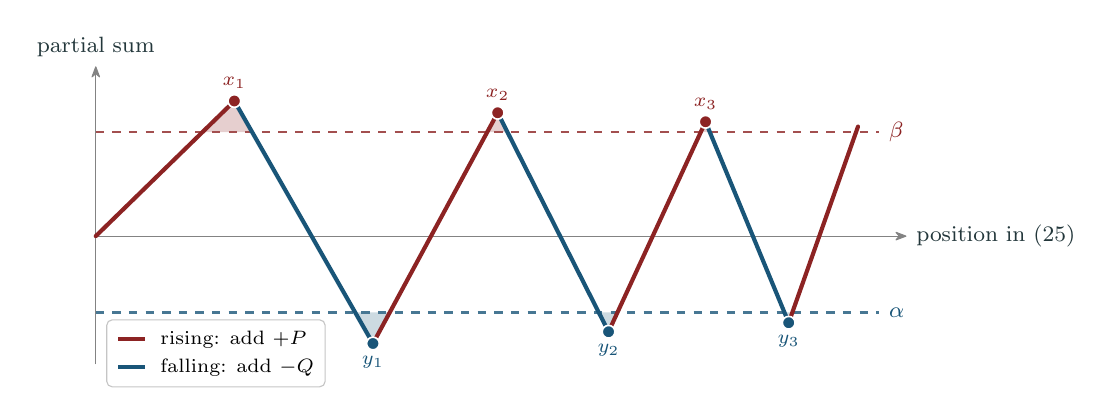
\begin{tikzpicture}[scale=0.88,
    >={Stealth[round]},
    rise/.style={thmcolor, line width=1.5pt, line cap=round, line join=round},
    fall/.style={defcolor, line width=1.5pt, line cap=round, line join=round},
    tp/.style={circle, draw=white, line width=0.6pt, inner sep=0pt, minimum size=4.6pt}]
    % --- Overshoot triangles (faint, drawn behind everything; they shrink) ---
    \fill[thmcolor!22] (1.538,1.5) -- (2.0,1.95) -- (2.257,1.5) -- cycle;
    \fill[thmcolor!22] (5.649,1.5) -- (5.8,1.78) -- (5.942,1.5) -- cycle;
    \fill[thmcolor!22] (8.731,1.5) -- (8.8,1.65) -- (8.862,1.5) -- cycle;
    \fill[defcolor!22] (3.743,-1.1) -- (4.0,-1.55) -- (4.243,-1.1) -- cycle;
    \fill[defcolor!22] (7.258,-1.1) -- (7.4,-1.38) -- (7.529,-1.1) -- cycle;
    \fill[defcolor!22] (9.938,-1.1) -- (10.0,-1.25) -- (10.053,-1.1) -- cycle;
    % --- Target lines ---
    \draw[dashed, thmcolor!80, line width=0.9pt] (0,1.5) -- (11.3,1.5)
      node[right, font=\footnotesize, text=thmcolor] {$\beta$};
    \draw[dashed, defcolor!80, line width=0.9pt] (0,-1.1) -- (11.3,-1.1)
      node[right, font=\footnotesize, text=defcolor] {$\alpha$};
    % --- Axes ---
    \draw[->, remcolor!75] (0,-1.85) -- (0,2.45)
      node[above, font=\footnotesize, text=mDarkTeal] {partial sum};
    \draw[->, remcolor!75] (0,0) -- (11.7,0)
      node[right, font=\footnotesize, text=mDarkTeal] {position in (25)};
    % --- Path: rising = add positive P's, falling = add negative Q's ---
    \draw[rise] (0,0) -- (2.0,1.95);
    \draw[fall] (2.0,1.95) -- (4.0,-1.55);
    \draw[rise] (4.0,-1.55) -- (5.8,1.78);
    \draw[fall] (5.8,1.78) -- (7.4,-1.38);
    \draw[rise] (7.4,-1.38) -- (8.8,1.65);
    \draw[fall] (8.8,1.65) -- (10.0,-1.25);
    \draw[rise] (10.0,-1.25) -- (11.0,1.58);
    % --- Turning points ---
    \node[tp, fill=thmcolor] at (2.0,1.95) {}; \node[font=\scriptsize, text=thmcolor, above=1pt] at (2.0,1.95) {$x_1$};
    \node[tp, fill=thmcolor] at (5.8,1.78) {}; \node[font=\scriptsize, text=thmcolor, above=1pt] at (5.8,1.78) {$x_2$};
    \node[tp, fill=thmcolor] at (8.8,1.65) {}; \node[font=\scriptsize, text=thmcolor, above=1pt] at (8.8,1.65) {$x_3$};
    \node[tp, fill=defcolor] at (4.0,-1.55) {}; \node[font=\scriptsize, text=defcolor, below=1pt] at (4.0,-1.55) {$y_1$};
    \node[tp, fill=defcolor] at (7.4,-1.38) {}; \node[font=\scriptsize, text=defcolor, below=1pt] at (7.4,-1.38) {$y_2$};
    \node[tp, fill=defcolor] at (10.0,-1.25) {}; \node[font=\scriptsize, text=defcolor, below=1pt] at (10.0,-1.25) {$y_3$};
    % --- Legend (in the empty lower-left corner; off the curve) ---
    \node[anchor=north west, align=left, font=\scriptsize, draw=remcolor!35,
      rounded corners=2pt, fill=white, inner sep=4pt] at (0.15,-1.20)
      {\textcolor{thmcolor}{\rule[0.4ex]{10pt}{1.3pt}}~~rising: add $+P$\\[2pt]
       \textcolor{defcolor}{\rule[0.4ex]{10pt}{1.3pt}}~~falling: add $-Q$};
  \end{tikzpicture}
  \end{center}

  \note{
    In this diagram, the horizontal axis is the position along the
    rearranged series, and the zigzag path tracks its partial sums. The
    red rising segments are stretches where we add positive capital "P"
    terms, climbing until the path crosses the upper red dashed line at
    beta; each crossing is a red dot, "x" sub 1, then "x" sub 2, then "x"
    sub 3. The blue falling segments are stretches where we add the
    negative capital "Q" terms, descending until the path crosses the
    lower blue dashed line at alpha, at the blue dots "y" sub 1, "y" sub
    2, "y" sub 3. Now look at the faint shaded triangles poking just above
    beta and just below alpha: those are the overshoots, and they clearly
    shrink as we move to the right. That shrinking is the whole game, and
    Step 4 makes it precise.
  }
\end{frame}

\begin{frame}{Proof of Theorem 3.54 --- Step 4: The Overshoots Vanish}
  \begin{proofblock}{Step 4: Turning points converge to $\beta$ and $\alpha$}
    Let $x_n$, $y_n$ be the partial sums of (25) whose last terms are
    $P_{m_n}$, $-Q_{k_n}$. Since $m_n$, $k_n$ were chosen \alert{smallest}:
    \[
      |x_n - \beta_n| \leq P_{m_n}, \qquad |y_n - \alpha_n| \leq Q_{k_n}.
    \]
    But $\Sigma a_n$ converges $\Rightarrow a_n \to 0 \Rightarrow
    P_n \to 0,\; Q_n \to 0$, so
    \[
      x_n \to \beta, \qquad y_n \to \alpha.
    \]
  \end{proofblock}

  \note{
    Step 4 measures the overshoots. Let "x" sub "n" denote the partial sum
    at the top of the "n"-th climb, the one ending with the term capital
    "P" sub "m" sub "n", and let "y" sub "n" be the partial sum at the
    bottom of the "n"-th descent. Here is where minimality pays off: since
    "m" sub "n" was the smallest index that pushed the sum past beta sub
    "n", the sum just before the final step was still at or below beta sub
    "n". So the overshoot of "x" sub "n" beyond beta sub "n" is at most
    that single last term. The same reasoning bounds "y" sub "n" near
    alpha sub "n". Now, the original series converges, so by Theorem 3.23
    its terms tend to zero, and hence both capital "P" sub "n" and capital
    "Q" sub "n" tend to zero. The overshoots are squeezed away: "x" sub
    "n" converges to beta and "y" sub "n" converges to alpha.
  }
\end{frame}

\begin{frame}{Proof of Theorem 3.54 --- Step 5: Conclusion}
  \begin{proofblock}{Step 5: No subsequential limit escapes $[\alpha, \beta]$}
    Between consecutive turning points, the partial sums of (25) move
    \alert{monotonically} --- so no number less than $\alpha$ or greater
    than $\beta$ can be a subsequential limit of the partial sums.
  \end{proofblock}

  \begin{hlbox}
  \[
    \boxed{\;\liminf_{n \to \infty} s'_n = \alpha, \qquad
           \limsup_{n \to \infty} s'_n = \beta\;} \tag{24}
  \]
  \end{hlbox}

  \hfill $\blacksquare$

  \note{
    One last check remains. We know the turning points converge to alpha
    and beta, so alpha and beta are subsequential limits of the partial
    sums. Could there be others, beyond them? No. Between consecutive
    turning points the partial sums move monotonically: climbing during a
    block of positive terms, falling during a block of negative terms. So
    every partial sum is trapped between a nearby "y" value and a nearby
    "x" value, and in the limit nothing can escape below alpha or above
    beta. Therefore the lower limit of the partial sums is exactly alpha
    and the upper limit is exactly beta, which is equation 24, and the
    proof is complete. After this chaos, the next theorem restores order.
  }
\end{frame}
}

{
\usebackgroundtemplate{%
  
\includegraphics[width=\paperwidth,height=\paperheight,keepaspectratio=false]{chapter_03_bg_05.png}%
}
% =============================================================================
\section{Absolute Convergence and Rearrangements}
% =============================================================================

\begin{frame}{Theorem 3.55: Absolute Convergence and Rearrangements}
  \begin{thmblock}{Theorem 3.55}
    If $\Sigma a_n$ is a series of \emph{complex} numbers which converges
    \alert{absolutely}, then \alert{every} rearrangement of $\Sigma a_n$
    converges, and they all converge to the \alert{same sum}.
  \end{thmblock}

  \vspace{0.5em}
  \begin{hlbox}
  \textbf{Contrast:}\\
  Conditionally convergent $\Rightarrow$ anything goes (3.54).\\
  Absolutely convergent $\Rightarrow$ \alert{order is irrelevant}.
  \end{hlbox}

  \note{
    Here is the positive counterpart, Theorem 3.55. If a series of complex
    numbers converges absolutely, then every rearrangement of it
    converges, and all rearrangements converge to the same sum. Note two
    upgrades compared with Riemann's theorem: the terms may now be
    complex, not just real, and the conclusion covers every rearrangement
    at once. The contrast at the bottom of the slide summarizes the
    dichotomy of this section: for conditionally convergent series,
    rearrangement can produce any behavior whatsoever; for absolutely
    convergent series, the order of the terms is completely irrelevant.
    The proof is short and elegant; it rests on the Cauchy criterion.
  }
\end{frame}

% --- Build 1/2 ---
\begin{frame}{Proof of Theorem 3.55}
  \begin{proofblock}{Step 1: Cauchy criterion for $\Sigma |a_n|$}
    Let $\Sigma a'_n$ be a rearrangement with partial sums $s'_n$. Given
    $\varepsilon > 0$, there exists $N$ such that $m \geq n \geq N$ implies
    \begin{equation}
      \sum_{i=n}^{m} |a_i| \leq \varepsilon. \tag{26}
    \end{equation}
  \end{proofblock}

  \note{
    Take any rearrangement, with partial sums "s" prime sub "n". Fix a
    positive epsilon. Since the series of absolute values converges, the
    Cauchy criterion, Theorem 3.22, applies to it: there is an index
    capital "N" beyond which every finite block of absolute values, from
    index "n" up to index "m", adds up to at most epsilon. That is
    equation 26 on the slide. In words: the total mass of the tail beyond
    capital "N" is tiny, no matter how many tail terms we grab and in
    what order. This is exactly the kind of control that conditionally
    convergent series lack. Now we put it to work.
  }
\end{frame}

% --- Build 2/2 ---
\begin{frame}{Proof of Theorem 3.55}
  \begin{proofblock}{Step 2: The head cancels, the tail is small}
    Choose $p$ so that $1, 2, \dots, N$ are all contained in
    $k_1, k_2, \dots, k_p$. For $n > p$:
    \[
      s_n - s'_n: \quad a_1, \dots, a_N \text{ \alert{cancel}}
      \;\Longrightarrow\;
      |s_n - s'_n| \leq \sum_{\substack{i > N \\ \text{finitely many} \\ \text{distinct}}} |a_i| \leq \varepsilon \quad \text{by (26)}.
    \]
    Hence $\{s'_n\}$ converges to the same sum as $\{s_n\}$. \hfill $\blacksquare$
  \end{proofblock}

  \note{
    Since the rearrangement uses every index exactly once, we can pick
    "p" so large that the first "p" rearranged terms include all of "a"
    sub 1 through "a" sub capital "N". Now compare the two partial sums
    for any "n" beyond "p". Both contain that entire head, so in the
    difference the head cancels completely. Whatever survives is a finite
    collection of terms with distinct indices, all larger than capital
    "N", and by equation 26 their combined size is at most epsilon. So
    the two partial sum sequences eventually travel within epsilon of
    each other; since "s" sub "n" converges, "s" prime sub "n" converges
    to the very same sum. The proof is complete.
  }
\end{frame}
}

{
\usebackgroundtemplate{%
  
\includegraphics[width=\paperwidth,height=\paperheight,keepaspectratio=false]{chapter_03_bg_06.png}%
}
% =============================================================================
\section{Summary}
% =============================================================================

% --- Build 1/3 ---
\begin{frame}{Summary}
  \begin{hlbox}
  \textbf{Key takeaways from this section:}
  \begin{small}
  \begin{itemize}
    \item \textbf{Rearrangement (3.52):} same terms, new order:
      $a'_n = a_{k_n}$, where $\{k_n\}$ is a permutation
    \item \textbf{Warning (3.53):} reordering alternating harmonic
      series \alert{changes the sum}
  \end{itemize}
  \end{small}
  \end{hlbox}

  \note{
    Let us review what we covered. A rearrangement, Definition 3.52, uses
    exactly the same terms as the original series, each exactly once, but
    visits them in a different order given by a permutation of the
    positive integers. Example 3.53 showed this is not a harmless
    operation: taking the alternating harmonic series and reordering it
    so that two positive terms precede each negative term produces a
    series whose partial sums eventually exceed five sixths, while the
    original sum lies below five sixths. Same ingredients, different sum.
    Next, the two main theorems.
  }
\end{frame}

% --- Build 2/3 ---
\begin{frame}{Summary}
  \begin{hlbox}
  \textbf{Key takeaways from this section:}
  \begin{small}
  \begin{itemize}
    \item \textbf{Rearrangement (3.52):} same terms, new order:
      $a'_n = a_{k_n}$, where $\{k_n\}$ is a permutation
    \item \textbf{Warning (3.53):} reordering alternating harmonic
      series \alert{changes the sum}
    \item \textbf{Riemann (3.54):} conditionally convergent real series:
      rearrangements achieve \alert{any} $\liminf = \alpha$, $\limsup = \beta$
  \end{itemize}
  \end{small}
  \end{hlbox}

  \note{
    The dramatic result is Riemann's rearrangement theorem, Theorem 3.54.
    For a real series that converges but not absolutely, the positive and
    negative parts are both divergent reservoirs, and a greedy
    construction lets us steer the partial sums across any pair of moving
    targets. The conclusion: any prescribed lower and upper limits alpha
    and beta can be achieved, so such a series can be rearranged to
    converge to any number we like, to diverge to either infinity, or to
    oscillate between any two bounds. The sum of a conditionally
    convergent series genuinely depends on the order of its terms.
  }
\end{frame}

% --- Build 3/3 ---
\begin{frame}{Summary}
  \begin{hlbox}
  \textbf{Key takeaways from this section:}
  \begin{small}
  \begin{itemize}
    \item \textbf{Rearrangement (3.52):} same terms, new order:
      $a'_n = a_{k_n}$, where $\{k_n\}$ is a permutation
    \item \textbf{Warning (3.53):} reordering alternating harmonic
      series \alert{changes the sum}
    \item \textbf{Riemann (3.54):} conditionally convergent real series:
      rearrangements achieve \alert{any} $\liminf = \alpha$, $\limsup = \beta$
    \item \textbf{Absolute convergence (3.55):} \alert{every} rearrangement
      converges to the \alert{same sum} --- order is irrelevant
  \end{itemize}
  \end{small}
  \end{hlbox}

  \begin{hlbox}
  \textbf{Coming up next:} Chapter 4 --- \emph{Continuity}.
  \end{hlbox}

  \note{
    The final takeaway is Theorem 3.55, the antidote to all this chaos:
    if a series converges absolutely, then every rearrangement converges,
    and all of them converge to the same sum. The Cauchy criterion makes
    the proof almost effortless, because the head of the series cancels
    in the comparison and the tail has small total mass regardless of
    order. This completes the dichotomy and also completes Chapter 3, our
    study of numerical sequences and series. In the next chapter we put
    sequences to work on a new subject: continuity. We will define
    limits of functions between metric spaces and connect continuity with
    the compactness and connectedness of Chapter 2. See you there.
  }
\end{frame}
}

\end{document}

